% !TeX root = ../thuthesis-example.tex

\chapter{引言}
对大部分的无人系统而言,为了让其能够自主完成任务,任务通常被分解为感知、决策、控制三个子任务,并要求在任务过程中有稳定的定位和通信。四旋翼飞行器是一种具有敏捷动作能力的飞行器,考虑到实际应用场景,飞行器往往需要具备自主感知和决策的能力以摆脱对外部定位、通信和操纵的依赖。在这种情况下四旋翼飞行器的自主导航是极具挑战性的系统问题。本研究借助强化学习这一交互式学习的人工智能算法,提出了一种三段式训练技术以解决复杂环境下四旋翼飞行器的自主导航问题,提升算法收敛速度,提高算法泛化性和飞行稳定性。同时本研究还针对算法训练和实机部署的需求开发了一整套仿真、部署平台。

下面将详细介绍研究背景,提出三个该领域现存的主要挑战并引出研究内容。最后介绍本研究报告各章节的构成。

\section{研究背景}
\label{background}
\subsection{四旋翼无人机发展背景}
四旋翼飞行器(quadrotor aircraft)是用四个旋翼产生升力的多轴飞行器,是直升机的一种。随着惯性测量单元(Inertial measurement unit, IMU)、飞行控制器(Flight control unit, FCU)和电子调速器(Electronic speed control, ESC)等电子器件的出现,四旋翼飞行器开始使用电传操纵系统控制,并逐渐发展为一种结构简单使用方便的飞行平台。四旋翼飞行器是迄今为止最为灵活、敏捷的无人飞行器之一\cite{verbeke2018experimental}\cite{ackermann2020ai}。得益于其敏捷的动力学特性,它们可以穿越复杂地形到达人类和大型机械无法到达的地方。四旋翼飞行器已经在搜索救援、物流、基础设施、娱乐、农业甚至军事领域得到了了广泛的应用。例如,美国国防部高级研究计划局(DARPA)在具备自主行动的无人机(集群)方向就先后设立了面向GPS拒止环境下的快速轻量级自主无人机(FLA)、面向未来复杂城市环境作战的进攻型机器人集群战术系统(OFFSET)、人机分层协作作战体系(ACE)等项目\cite{darpa2023}。

相较于其它无人系统,四旋翼飞行器在执行自主任务时具有以下三个显著特点:
\begin{enumerate}
  \item 载荷资源受限。四旋翼飞行器作为一种空中无人平台,在任务目标和续航时间确定的情况下,其载荷资源受严格限制。飞行器所搭载的传感、计算、通信设备受载荷限制影响,其提供的感知、通信质量往往比其他无人系统更低。
  \item 计算资源受限。在载荷首先的前提下,机载计算机的规模严格受限,同时考虑到功率的限制,机载计算机的计算能力往往远低于同一时代的消费级计算机。
  \item 动力学高度复杂。相较于无人车和其它飞行器,四旋翼无人机的动力学高度复杂且非线性。同时由于其飞行特性,四旋翼无人机对决策、控制的稳定性和连续性都有较高要求。
\end{enumerate}
在上述情况下,自主导航任务对算法提出了更高要求,感知算法需要对传感器噪声、运动带来的模糊和不断变化的环境具有鲁棒性,而决策和控制算法需要在包含噪声的感知结果下利用有限的计算资源做出稳定而有效的规划。现有较成熟的方法可大致分为两类:基于优化的方法和基于学习的方法,详细的介绍将在章节\ref{ralated_works}中展开。

\subsection{强化学习发展背景}
强化学习(Reinforcement learning, RL)是机器学习的一个分支。其工作流程是智能体(Agent)在与环境(Environment)交互的过程中不断获得奖励(Reward),通过试错的方式学习到最优策略(Policy)。其工作原理如图\ref{fig_RL}所示。深度学习(Deep learning, DL)具有学习特征表示的梯度信息,而强化学习算法可以利用环境信息产生梯度并学习最佳策略。二者结合的方法被称为深度强化学习,已在各个领域取得了很多成就。例如2016年谷歌开发的AlphaGo在围棋人机大赛中战胜世界冠军李世石,标志着人工智能又一里程碑式的胜利。而后该团队推陈出新,提出了在不使用人类棋局数据情况下战胜AlphaGo的AlphaZero、在StarCraft \uppercase\expandafter{\romannumeral2}中战胜职业玩家的AlphaStar、可以预测蛋白质结构的AlphaFold、可以高效计算矩阵乘法的AlphaTensor等AI。同时,深度强化学习在无人驾驶、机器人控制、自然语言处理等领域也取得了很多成果。深度强化学习相比其他方法,具有以下三个显著优势:

\begin{figure}
  \centering
  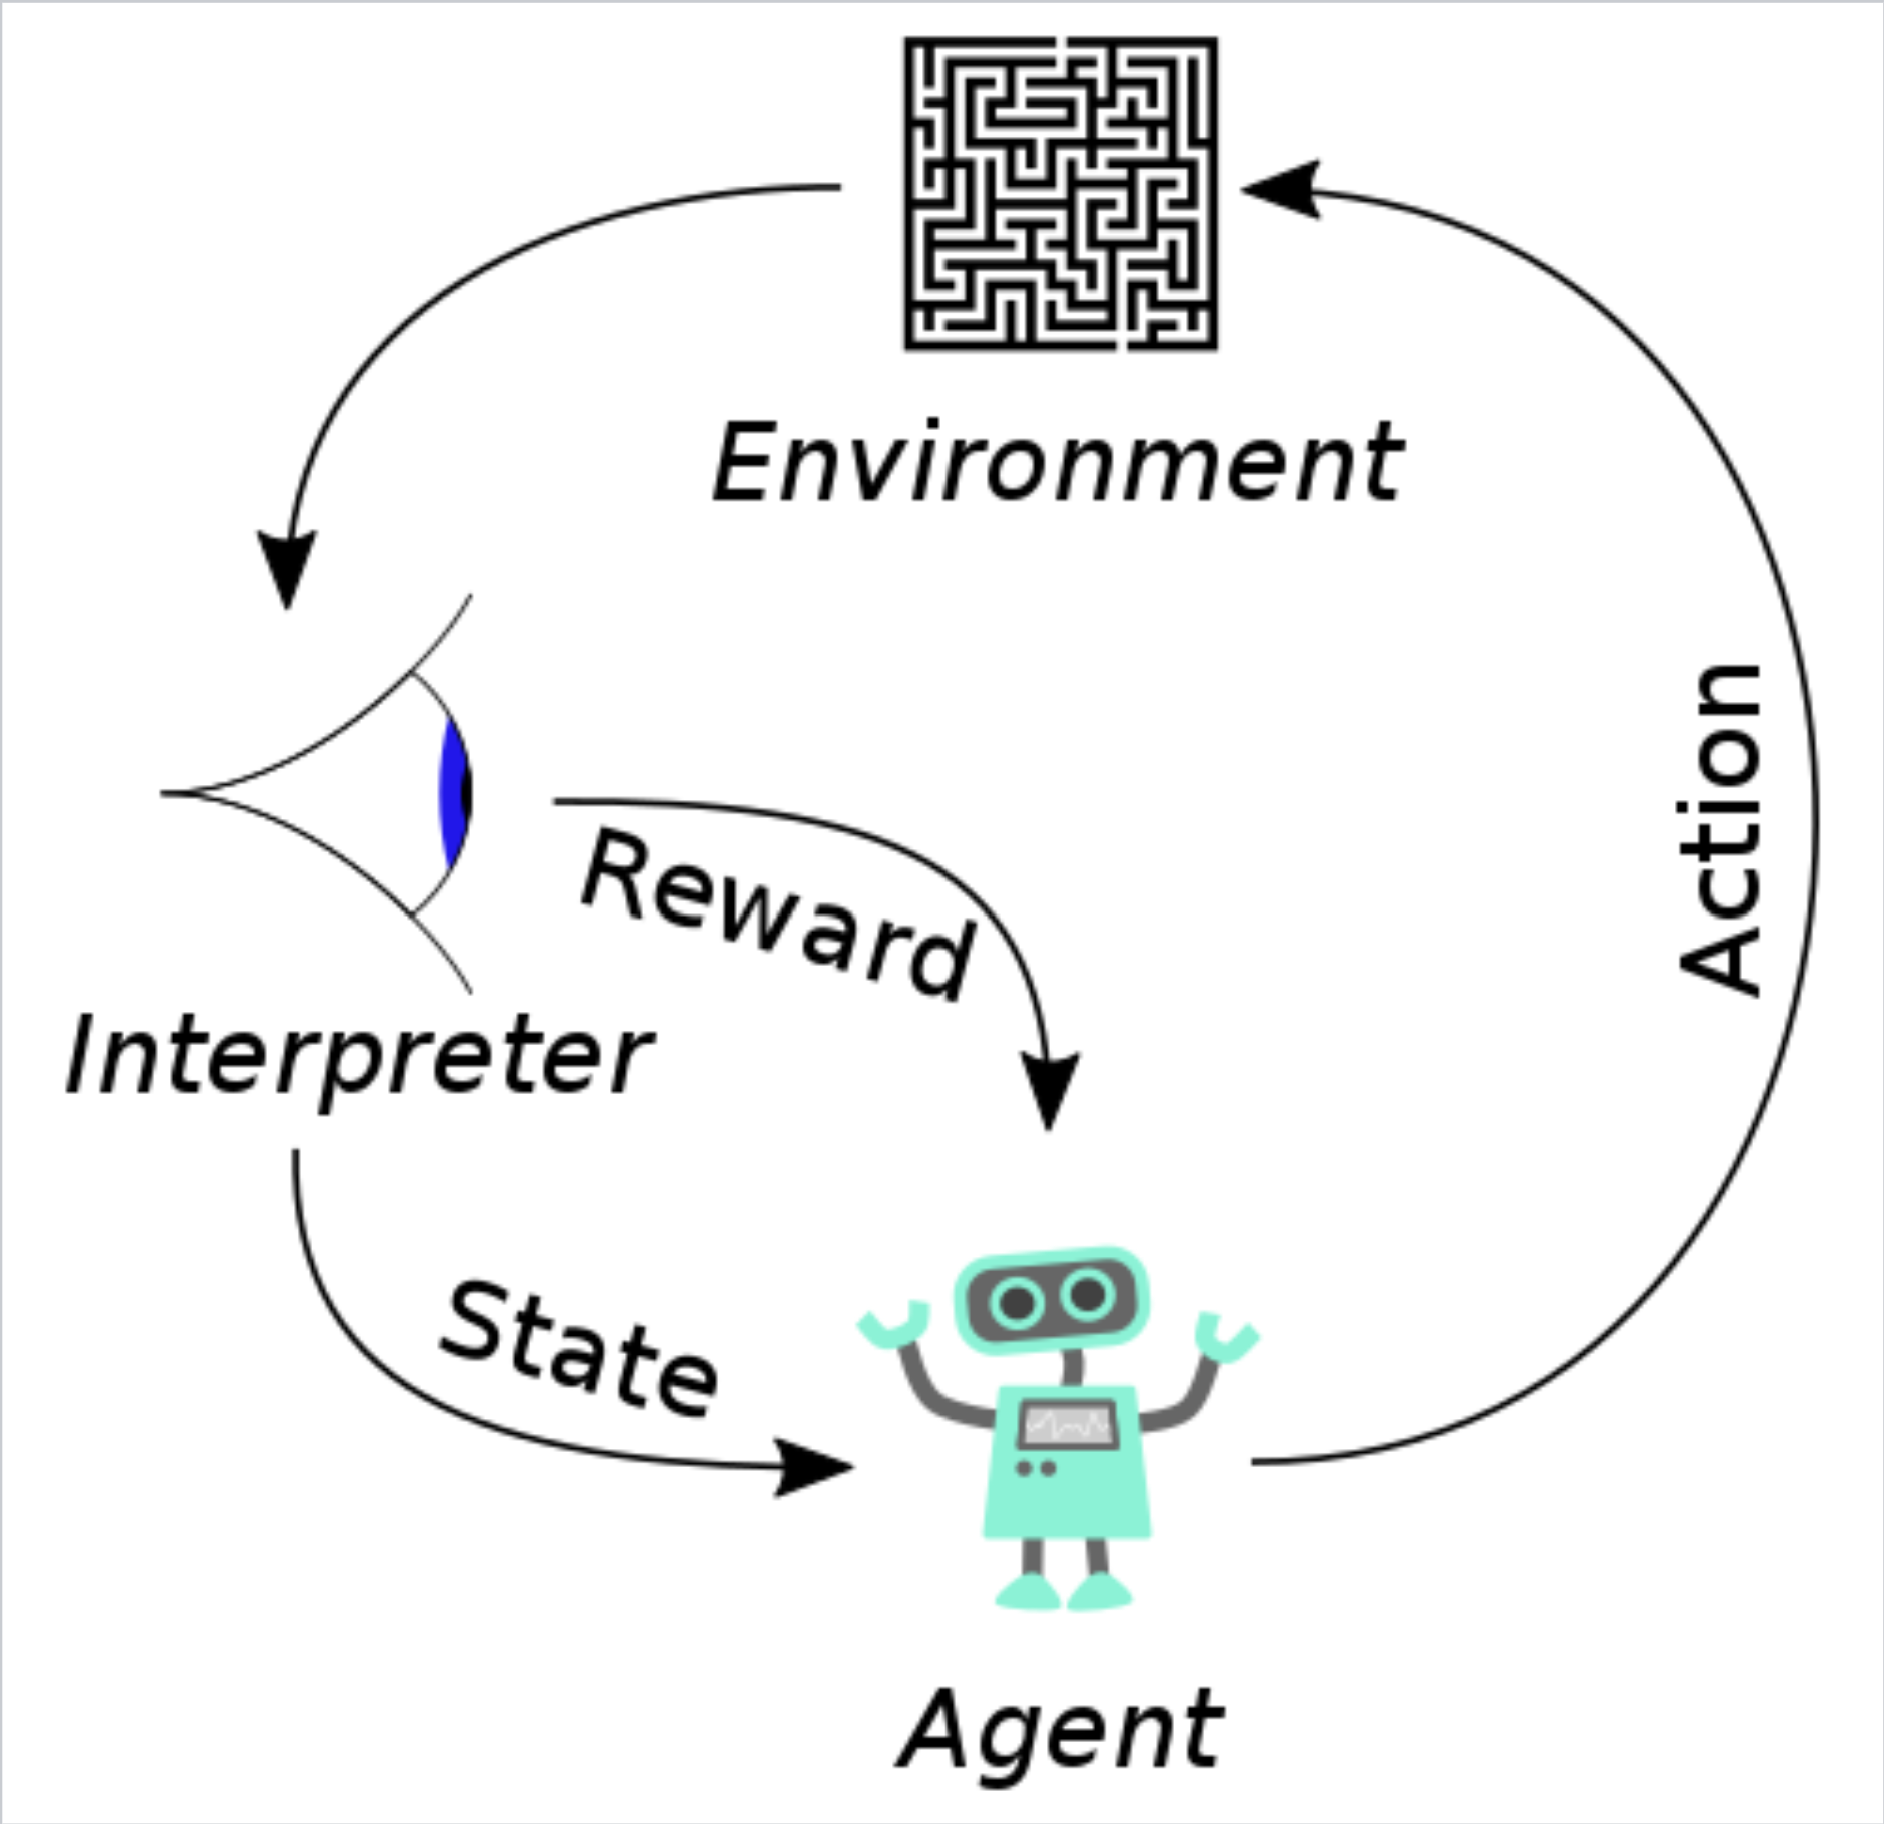
\includegraphics[width = 0.6\textwidth]{RL.png}
  \caption{强化学习工作原理}
  \label{fig_RL}
\end{figure}

\section{相关工作}
\label{ralated_works}

\section{研究目的}

\section{各章节概述}

% \section{引言的写法}

% 一篇学位论文的引言大致包含如下几个部分:
% 1、问题的提出;
% 2、选题背 景及意义;
% 3、文献综述;
% 4、研究方法;
% 5、论文结构安排。
% \begin{itemize}
%   \item 问题的提出:要清晰地阐述所要研究的问题“是什么”。
%     \footnote{选题时切记要有“问题意识”,不要选不是问题的问题来研究。}
%   \item 选题背景及意义:论述清楚为什么选择这个题目来研究,即阐述该研究对学科发展的贡献、对国计民生的理论与现实意义等。
%   \item 文献综述:对本研究主题范围内的文献进行详尽的综合述评,“述”的同时一定要有“评”,指出现有研究状态,仍存在哪些尚待解决的问题,讲出自己的研究有哪些探索性内容。
%   \item 研究方法:讲清论文所使用的学术研究方法。
%   \item 论文结构安排:介绍本论文的写作结构安排。
% \end{itemize}



% \section{正文的写法}

% 本部分是论文作者的研究内容,不能将他人研究成果不加区分地掺和进来。
% 已经在引言的文献综述部分讲过的内容,这里不需要再重复。
% 各章之间要存在有机联系,符合逻辑顺序。



% \section{结论的写法}

% 结论是对论文主要研究结果、论点的提炼与概括,应精炼、准确、完整,使读者看后能全面了解论文的意义、目的和工作内容。
% 结论是最终的、总体的结论,不是正文各章小结的简单重复。
% 结论应包括论文的核心观点,主要阐述作者的创造性工作及所取得的研究成果在本领域中的地位、作用和意义,交代研究工作的局限,提出未来工作的意见或建议。
% 同时,要严格区分自己取得的成果与指导教师及他人的学术成果。

% 在评价自己的研究工作成果时,要实事求是,除非有足够的证据表明自己的研究是“首次”、“领先”、“填补空白”的,否则应避免使用这些或类似词语。
